\documentclass[a4paper,11pt]{article}
\usepackage[dvipsnames,table]{xcolor}
\usepackage[a4paper,margin=2.5cm,headheight=15pt]{geometry}
\usepackage[utf8]{inputenc}
\usepackage[T1]{fontenc}
\usepackage[serbian]{babel}
\usepackage{lmodern,microtype}
\usepackage{amsmath,amssymb,mathtools}
\numberwithin{equation}{section}
\usepackage{graphicx,adjustbox,placeins}
\graphicspath{{Images/}}
\usepackage{booktabs,tabularx,longtable,array,multirow,makecell}
\usepackage{caption,subcaption}
\captionsetup{font=small,labelfont=bf}
\usepackage{siunitx}
\sisetup{detect-all}
\usepackage[most]{tcolorbox}
\usepackage{enumitem}
\setlist{nosep}
\usepackage{fancyhdr}
\definecolor{Primary}{HTML}{1F77B4}
\definecolor{Accent}{HTML}{2CA02C}
\usepackage[colorlinks=true,linkcolor=Primary,citecolor=Primary,urlcolor=Primary]{hyperref}
\usepackage{cleveref}
\pagestyle{fancy}
\fancyhf{}
\lhead{\small\textit{Aritmetičke operacije}}
\rhead{\thepage}
\renewcommand{\arraystretch}{1.25}
\newcolumntype{C}{>{\centering\arraybackslash}X}
\renewcommand{\contentsname}{Sadržaj}
\setlength{\emergencystretch}{2em}
\allowdisplaybreaks[2]
\newcommand{\napomena}[1]{\begin{tcolorbox}[colback=gray!10,colframe=black,boxrule=0.5pt,breakable]#1\end{tcolorbox}}
\newcommand{\redlinija}{\arrayrulecolor{black!28}\specialrule{0.3pt}{2pt}{2pt}\arrayrulecolor{black}}
\newcommand{\kod}[1]{\ensuremath{\mathtt{#1}}}
\begin{document}
\hypersetup{pageanchor=false}
\begin{titlepage}
\thispagestyle{empty}
\begin{center}
{\Large\bfseries UNIVERZITET U BEOGRADU -- ELEKTROTEHNIČKI FAKULTET\\ KATEDRA ZA ELEKTRONIKU\par}
\vspace{25mm}
{\LARGE\bfseries DIGITALNA ELEKTRONIKA 1\par}
\vspace{2mm}
{\large Materijali za računske vežbe\par}
\vspace{18mm}
{\Large\bfseries ARITMETIČKE OPERACIJE\par}
\vspace{3mm}
{\large Vežbe 4\par}
\vfill
\begin{minipage}{0.62\linewidth}
\raggedright\textbf{Autori:}\\[4pt]\small
\begin{tabular}{@{}ll@{}}
Nikola Petrović & \href{mailto:p.z.nikola@etf.bg.ac.rs}{\texttt{p.z.nikola@etf.bg.ac.rs}}\\
Haris Turkmanović & \href{mailto:haris@etf.bg.ac.rs}{\texttt{haris@etf.bg.ac.rs}}\\
\end{tabular}
\end{minipage}\hfill
\begin{minipage}{0.34\linewidth}\raggedleft Beograd, \today\end{minipage}
\end{center}
\end{titlepage}
\hypersetup{pageanchor=true}
\tableofcontents
\newpage

% Izvor DOCX: blok 31
\FloatBarrier
\section{Uvod}\label{sec:1}


% Izvor DOCX: blok 32
\FloatBarrier
\subsection{Sabiranje i oduzimanje neoznačenih brojeva}\label{sec:1.1}


% Izvor DOCX: blok 33
Sabiranje neoznačenih brojeva X = \emph{x}\textsubscript{n} \emph{x}\textsubscript{n-1} \emph{x}\textsubscript{n-2} \ldots{} \emph{x}\textsubscript{1} \emph{x}\textsubscript{0} i Y = \emph{y}\textsubscript{n} \emph{y}\textsubscript{n-1} \emph{y}\textsubscript{n-2} \ldots{} \emph{y}\textsubscript{1} \emph{y}\textsubscript{0} u brojnom sistemu sa osnovom \emph{r} se realizuje sabiranjem svake od cifara brojeva X i Y u brojnom sistemu \emph{r}, počevši od cifre najmanje težine, i dodavanjem cifara ulaznog prenosa . Dakle, cifra \emph{s}\textsubscript{i} zbira S se određuje primenom sledeće formule:



% Izvor DOCX: blok 34
\begin{equation}\label{eq:1.1.1}
s_{i} = \left( x_{i}\  + \ y_{i}\  + c_{i} \right)\ mod\ r
\end{equation}


% Izvor DOCX: blok 35
\begin{center}\begin{adjustbox}{max width=\linewidth}
\begin{tabular}{ccccccc}\toprule
\emph{c}\textsubscript{n+1} & \emph{c}\textsubscript{n} & \emph{c}\textsubscript{n-1} & \emph{c}\textsubscript{n-2} & \ldots{} & \emph{c}\textsubscript{1} & \emph{c}\textsubscript{0} \\
\midrule
+ & \emph{x}\textsubscript{n} & \emph{x}\textsubscript{n-1} & \emph{x}\textsubscript{n-2} & \ldots{} & \emph{x}\textsubscript{1} & \emph{x}\textsubscript{0} \\
\redlinija
 & y\textsubscript{n} & y\textsubscript{n-1} & \emph{y}\textsubscript{n-2} & \ldots{} & \emph{y}\textsubscript{1} & \emph{y}\textsubscript{0} \\
\redlinija
s\textsubscript{n+1} & s\textsubscript{n} & s\textsubscript{n-1} & \emph{s}\textsubscript{n-2} & \ldots{} & \emph{s}\textsubscript{1} & \emph{s}\textsubscript{0} \\
\bottomrule\end{tabular}\end{adjustbox}\end{center}


% Izvor DOCX: blok 36
Ulazni prenos je $c_i$. Izlazni prenos je $c_{i+1}=1$ ako je $x_i+y_i+c_i\ge r$, a inače je nula.

% Izvor DOCX: blok 37
U slučaju da brojevi X i Y nisu predstavljeni sa istim brojem cifara, pre realizacije operacije sabiranja potrebno je dodati vodeće nule ispred sabirka koji ima manje cifara kako bi se broj cifara izjednačio. Ukoliko sabirci X i Y sadrže razlomljeni deo, pre realizacije operacije sabiranja neophodno je poravnati decimalne tačke sabiraka.



% Izvor DOCX: blok 38
Oduzimanje neoznačenih brojeva X = \emph{x}\textsubscript{n} \emph{x}\textsubscript{n-1} \emph{x}\textsubscript{n-2} \ldots{} \emph{x}\textsubscript{1} \emph{x}\textsubscript{0} i Y = \emph{y}\textsubscript{n} \emph{y}\textsubscript{n-1} \emph{y}\textsubscript{n-2} \ldots{} \emph{y}\textsubscript{1} \emph{y}\textsubscript{0} u brojnom sistemu sa osnovom \emph{r} se realizuje oduzimanjem svake od cifara brojeva X i Y u brojnom sistemu \emph{r}, počevši od cifre najmanje težine, i oduzimanjem cifara ulazne pozajmice. Dakle, cifra \emph{d}\textsubscript{i} razlike D se određuje primenom sledeće formule:



% Izvor DOCX: blok 39
\begin{equation}\label{eq:1.2.1}
d_{i} = \left( x_{i} - \ y_{i} - b_{i} \right)\ mod\ r
\end{equation}


% Izvor DOCX: blok 40
\begin{center}\begin{adjustbox}{max width=\linewidth}
\begin{tabular}{ccccccc}\toprule
\emph{b}\textsubscript{n+1} & \emph{b}\textsubscript{n} & \emph{b}\textsubscript{n-1} & \emph{b}\textsubscript{n-2} & \ldots{} & \emph{b}\textsubscript{1} & \emph{b}\textsubscript{0} \\
\midrule
 & \emph{x}\textsubscript{n} & \emph{x}\textsubscript{n-1} & \emph{x}\textsubscript{n-2} & \ldots{} & \emph{x}\textsubscript{1} & \emph{x}\textsubscript{0} \\
\redlinija
- & \emph{y}\textsubscript{n} & \emph{y}\textsubscript{n-1} & \emph{y}\textsubscript{n-2} & \ldots{} & \emph{y}\textsubscript{1} & \emph{y}\textsubscript{0} \\
\redlinija
\emph{d}\textsubscript{n+1} & \emph{d}\textsubscript{n} & \emph{d}\textsubscript{n-1} & \emph{d}\textsubscript{n-2} & \ldots{} & \emph{d}\textsubscript{1} & \emph{d}\textsubscript{0} \\
\bottomrule\end{tabular}\end{adjustbox}\end{center}


% Izvor DOCX: blok 41
Ulazna pozajmica je $b_i$. Izlazna pozajmica je $b_{i+1}=1$ ako je $x_i-y_i-b_i<0$, a inače je nula. Početna pozajmica je $b_0$, dok $b_{n+1}=1$ označava da je umanjenik manji od umanjioca (uz ulaznu pozajmicu).

% Izvor DOCX: blok 42
Pre oduzimanja izjednačavamo broj cifara vodećim nulama i poravnavamo tačke. Ako je umanjenik manji od umanjioca, matematička razlika je negativna i nije predstavljiva kao neoznačen broj; zapis na ograničenoj širini predstavlja ostatak modulo $r^N$.

% Izvor DOCX: blok 43
\FloatBarrier
\subsection{Aritmetičke operacije u predstavi znak i apsolutna vrednost}\label{sec:1.2}


% Izvor DOCX: blok 44
Prilikom aritmetičkih operacija sa brojevima X = \emph{x}\textsubscript{n} \emph{x}\textsubscript{n-1} \emph{x}\textsubscript{n-2} \ldots{} \emph{x}\textsubscript{1} \emph{x}\textsubscript{0} i Y = \emph{y}\textsubscript{n} \emph{y}\textsubscript{n-1} \emph{y}\textsubscript{n-2} \ldots{} \emph{y}\textsubscript{1} \emph{y}\textsubscript{0}, koji su dati u predstavi znak i apsolutna vrednost, najpre je neophodno odrediti znak rezultata a zatim primeniti neku od odgovarajućih operacija nad apsolutnim vrednostima brojeva X i Y.



% Izvor DOCX: blok 45
Za sabiranje brojeva istog znaka sabiraju se apsolutne vrednosti i zadržava znak. Za suprotne znake oduzima se manja apsolutna vrednost od veće, a znak se preuzima od operanda veće apsolutne vrednosti. Oduzimanje $X-Y$ svodi se na $X+(-Y)$. Tvrdnja da iz $|X|<|Y|$ sledi $X-Y<0$ važi kada su $X$ i $Y$ nenegativni; nije opšte pravilo za označene operande.

% Izvor DOCX: blok 46
\FloatBarrier
\subsection{Sabiranje i oduzimanje brojeva u komplementu osnove}\label{sec:1.3}


% Izvor DOCX: blok 47
Sabiranje u komplementu osnove izvodi se cifru po cifru, posle proširenja znaka na zadatu širinu $N$. Zadržava se $N$ cifara rezultata, tj. računa se modulo $r^N$. Kod zapisa sa $k$ razlomljenih cifara tačka se poravnava, a korak je $r^{-k}$.

% Izvor DOCX: blok 48
I neoznačena i označena aritmetika imaju ograničen opseg. Kod neoznačenog sabiranja prekoračenje označava izlazni prenos. Kod označenog sabiranja prekoračenje (OF) postoji ako tačan zbir izlazi iz opsega zadate predstave; za binarni KO to je slučaj kada su sabirci istog, a rezultat suprotnog znaka. Ekvivalentno, $\mathrm{OF}=c_{n+1}\oplus c_n$, gde je $n$ indeks bita znaka.

% Izvor DOCX: blok 49
\begin{center}\begin{adjustbox}{max width=\linewidth}
\begin{tabular}{ccccccc}\toprule
\emph{c}\textsubscript{n+1} & \emph{c}\textsubscript{n} & \emph{c}\textsubscript{n-1} & \emph{c}\textsubscript{n-2} & \ldots{} & \emph{c}\textsubscript{1} & \emph{c}\textsubscript{0} \\
\midrule
 & \emph{x}\textsubscript{n} & \emph{x}\textsubscript{n-1} & \emph{x}\textsubscript{n-2} & \ldots{} & \emph{x}\textsubscript{1} & \emph{x}\textsubscript{0} \\
\redlinija
+ & \emph{y}\textsubscript{n} & \emph{y}\textsubscript{n-1} & \emph{y}\textsubscript{n-2} & \ldots{} & \emph{y}\textsubscript{1} & \emph{y}\textsubscript{0} \\
\redlinija
{\emph{s}\textsubscript{n+1}} & \emph{s}\textsubscript{n} & \emph{s}\textsubscript{n-1} & \emph{s}\textsubscript{n-2} & \ldots{} & \emph{s}\textsubscript{1} & \emph{s}\textsubscript{0} \\
\bottomrule\end{tabular}\end{adjustbox}\end{center}


% Izvor DOCX: blok 50
Oduzimanje brojeva u komplementu osnove se svodi na sabiranje u komplementu osnove gde se umesto umanjioca uzima njegova suprotna vrednost.



% Izvor DOCX: blok 51
\FloatBarrier
\subsection{Sabiranje i oduzimanje brojeva u komplementu maksimalne vrednosti}\label{sec:1.4}


% Izvor DOCX: blok 52
Sabiranje u komplementu maksimalne vrednosti izvodi se cifru po cifru. Izlazni prenos dodaje se na cifru najmanje težine (kružni prenos). Kod razlomljenih zapisa to znači dodavanje jedinice poslednjeg mesta, a ne celog broja 1.

% Izvor DOCX: blok 53
\begin{center}\begin{adjustbox}{max width=\linewidth}
\begin{tabular}{ccccccc}\toprule
\emph{c}\textsubscript{n+1} & \emph{c}\textsubscript{n} & \emph{c}\textsubscript{n-1} & \emph{c}\textsubscript{n-2} & \ldots{} & \emph{c}\textsubscript{1} & \emph{c}\textsubscript{0} \\
\midrule
 & \emph{x}\textsubscript{n} & \emph{x}\textsubscript{n-1} & \emph{x}\textsubscript{n-2} & \ldots{} & \emph{x}\textsubscript{1} & \emph{x}\textsubscript{0} \\
\redlinija
+ & \emph{y}\textsubscript{n} & \emph{y}\textsubscript{n-1} & \emph{y}\textsubscript{n-2} & \ldots{} & \emph{y}\textsubscript{1} & \emph{y}\textsubscript{0} \\
\redlinija
\emph{t}\textsubscript{n+1} & \emph{t}\textsubscript{n} & \emph{t}\textsubscript{n-1} & \emph{t}\textsubscript{n-2} & \ldots{} & \emph{t}\textsubscript{1} & \emph{t}\textsubscript{0} \\
\redlinija
 &  &  &  &  &  & \emph{t}\textsubscript{n+1} \\
\redlinija
 & \emph{s}\textsubscript{n} & \emph{s}\textsubscript{n-1} & \emph{s}\textsubscript{n-2} & \ldots{} & \emph{s}\textsubscript{1} & \emph{s}\textsubscript{0} \\
\bottomrule\end{tabular}\end{adjustbox}\end{center}


% Izvor DOCX: blok 54
Oduzimanje označenih brojeva u komplementu maksimalne vrednosti se najčešće vrši svođenjem na sabiranje brojeva u komplementu maksimalne vrednosti tako što se umanjilac zameni njegovom suprotnom vrednošću u komplementu maksimalne vrednosti a zatim sabere sa umanjenikom.



% Izvor DOCX: blok 55
\FloatBarrier
\subsection{Množenje neoznačenih brojeva}\label{sec:1.5}


% Izvor DOCX: blok 56
Pri množenju neoznačenih brojeva najpre privremeno uklanjamo tačke i množimo celobrojne kodne reči. Ako operandi imaju $k_X$ i $k_Y$ razlomljenih cifara, proizvod ima $k_X+k_Y$ razlomljenih cifara.

% Izvor DOCX: blok 57
Iako je prvi način zastupljeniji u slučaju standardnog množenja u decimalnom brojnom sistemu, takav pristup dovoljno tačno ne oslikava implementaciju množenja u digitalnoj logici. Alternativa, koja je pogodnija za implementaciju u digitalnoj logici, podrazumeva postupno određivanje međurezultata sabiranja.



% Izvor DOCX: blok 58
\FloatBarrier
\subsection{Množenje označenih brojeva}\label{sec:1.6}


% Izvor DOCX: blok 59
Za binarni KO broj $Y$ širine $N$ ima vrednost
\[Y=-y_{N-1}2^{N-1}+\sum_{i=0}^{N-2}y_i2^i.\]
Zato poslednji parcijalni proizvod ima negativnu težinu, dok se ostali sabiraju. Pre pomeranja i sabiranja svaki parcijalni proizvod proširuje se znakom na širinu rezultata; za dva $N$-bitna operanda puna širina proizvoda je $2N$. U međukoracima se ne sme izgubiti bit potreban za konačan rezultat. Za razlomljene operande na kraju vraćamo tačku. Pravilo o prostom negiranju poslednjeg parcijalnog proizvoda odnosi se na binarni KO; nije opšti algoritam za sve osnove i predstave.

% Izvor DOCX: blok 60
\FloatBarrier
\subsection{Deljenje neoznačenih brojeva}\label{sec:1.7}


% Izvor DOCX: blok 61
Operacija deljenja neoznačenih binarnih brojeva se realizuje na isti način kao operacija deljenja neoznačenih decimalnih brojeva


\napomena{U zadacima sa označenim brojevima svaki operand najpre se tumači na svojoj izvornoj širini. Zatim se proširuje na širinu rezultata, uz očuvanje vrednosti. Za $R=r^N$ i celobrojnu kodnu reč $U$, KO ima vrednost $U$ kada je $U<\lceil R/2\rceil$, a inače $U-R$. Za KMV uzimamo simetričan opseg $[-\lfloor(R-2)/2\rfloor,\lfloor(R-2)/2\rfloor]$, sa obe nule; negativna vrednost ima kod $R-1-|D|$. Kada je $r$ neparno, srednja samokomplementarna reč $(R-1)/2$ se ne koristi. Za $k$ razlomljenih cifara sve vrednosti skaliraju se sa $r^{-k}$. Ova konvencija uklanja neodređenost primera u osnovi 7.}

% Izvor DOCX: blok 62
\FloatBarrier
\section{Zadaci sa časova vežbi}\label{sec:2}


% Izvor DOCX: blok 63
\FloatBarrier
\subsection{Zadatak 1}\label{sec:2.1}


% Izvor DOCX: blok 64
\begin{enumerate}[label=\alph*),start=1,leftmargin=*]
\item Izvršiti sabiranje neoznačenih brojeva brojnom u sistemu sa osnovom u kome su dati i odrediti sve cifre prenosa:

\end{enumerate}


% Izvor DOCX: blok 65
100.11\textsubscript{2} + 10.01\textsubscript{2}, 11111\textsubscript{2} + 10011\textsubscript{2} uz ulazni prenos 1, 294\textsubscript{10} + 42\textsubscript{10}, 5325\textsubscript{7} + 4163\textsubscript{7}, AF3.50\textsubscript{16} + FB2.B9\textsubscript{16}, 26417\textsubscript{8} + 13140\textsubscript{8}



% Izvor DOCX: blok 66
b) Izvršiti oduzimanje neoznačenih brojeva u osnovi u kojoj su dati i odrediti sve cifre pozajmice:

% Izvor DOCX: blok 67
110101\textsubscript{2} - 10110\textsubscript{2}, 100010\textsubscript{2} - 10010\textsubscript{2} uz ulaznu pozajmicu 1, 25.2\textsubscript{10} - 2.8\textsubscript{10}, 436\textsubscript{8} - 627\textsubscript{8}, FB.2B9\textsubscript{16} - AF.350\textsubscript{16}, 26417\textsubscript{8} - 13140\textsubscript{8}



% Izvor DOCX: blok 68
\subsubsection*{Rešenje:}


% Izvor DOCX: blok 69
\begin{enumerate}[label=\alph*),start=1,leftmargin=*]
\item Na osnovu algoritma opisanog u \ref{sec:1.1} važi:

\end{enumerate}


% Izvor DOCX: blok 70
\begin{longtable}{p{0.33\linewidth} p{0.36\linewidth} p{0.23\linewidth}}\toprule
Izraz & Postupak & Rezultat\\\midrule\endhead
$(100.11)_{2}+(10.01)_{2}$ & $\begin{array}{r}\text{c}:\ 000110\\100.11\\+010.01\\\hline 111.00\end{array}$ & $111.00$\\[5pt]
\redlinija
$(11111)_{2}+(10011)_{2}+1$ & $\begin{array}{r}\text{c}:\ 111111\\11111\\+10011\\\hline 10011\end{array}$ & $110011$\\[5pt]
\redlinija
$(294)_{10}+(42)_{10}$ & $\begin{array}{r}\text{c}:\ 0100\\294\\+042\\\hline 336\end{array}$ & $336$\\[5pt]
\redlinija
$(5325)_{7}+(4163)_{7}$ & $\begin{array}{r}\text{c}:\ 10110\\5325\\+4163\\\hline 2521\end{array}$ & $12521$\\[5pt]
\redlinija
$(AF3.50)_{16}+(FB2.B9)_{16}$ & $\begin{array}{r}\text{c}:\ 110100\\AF3.50\\+FB2.B9\\\hline AA6.09\end{array}$ & $1AA6.09$\\[5pt]
\redlinija
$(26417)_{8}+(13140)_{8}$ & $\begin{array}{r}\text{c}:\ 010000\\26417\\+13140\\\hline 41557\end{array}$ & $41557$\\[5pt]
\bottomrule\end{longtable}


% Izvor DOCX: blok 71
\begin{enumerate}[label=\alph*),start=2,leftmargin=*]
\item Na osnovu algoritma opisanog u \ref{sec:1.1} važi:

\end{enumerate}


% Izvor DOCX: blok 72
\begin{longtable}{p{0.33\linewidth} p{0.36\linewidth} p{0.23\linewidth}}\toprule
Izraz & Postupak & Rezultat\\\midrule\endhead
$(110101)_{2}-(10110)_{2}$ & $\begin{array}{r}\text{b}:\ 0111100\\110101\\-010110\\\hline 011111\end{array}$ & $\begin{array}{r}011111\\b_{N}=0\end{array}$\\[5pt]
\redlinija
$(100010)_{2}-(10010)_{2}-1$ & $\begin{array}{r}\text{b}:\ 0111111\\100010\\-010010\\\hline 001111\end{array}$ & $\begin{array}{r}001111\\b_{N}=0\end{array}$\\[5pt]
\redlinija
$(25.2)_{10}-(2.8)_{10}$ & $\begin{array}{r}\text{b}:\ 0010\\25.2\\-02.8\\\hline 22.4\end{array}$ & $\begin{array}{r}22.4\\b_{N}=0\end{array}$\\[5pt]
\redlinija
$(436)_{8}-(627)_{8}$ & $\begin{array}{r}\text{b}:\ 1010\\436\\-627\\\hline 607\end{array}$ & $\begin{array}{r}-171\\b_{N}=1\end{array}$\\[5pt]
\redlinija
$(FB.2B9)_{16}-(AF.350)_{16}$ & $\begin{array}{r}\text{b}:\ 011000\\FB.2B9\\-AF.350\\\hline 4B.F69\end{array}$ & $\begin{array}{r}4B.F69\\b_{N}=0\end{array}$\\[5pt]
\redlinija
$(26417)_{8}-(13140)_{8}$ & $\begin{array}{r}\text{b}:\ 000100\\26417\\-13140\\\hline 13257\end{array}$ & $\begin{array}{r}13257\\b_{N}=0\end{array}$\\[5pt]
\bottomrule\end{longtable}

Redovi označeni sa $c$ ili $b$ čitaju se od izlaznog prenosa/pozajmice $c_N$ ili $b_N$ do početnog $c_0$ ili $b_0$. Kod negativne neoznačene razlike poslednji red postupka prikazuje modularni ostatak, a kolona rezultata matematičku razliku.\par

% Izvor DOCX: blok 73
\FloatBarrier
\subsection{Zadatak 2}\label{sec:2.2}


% Izvor DOCX: blok 74
\begin{enumerate}[label=\alph*),start=1,leftmargin=*]
\item Izvršiti sledeće operacije u kodu znak i apsolutna vrednost ako je na raspolaganju dovoljan broj bita:

\end{enumerate}


% Izvor DOCX: blok 75
A + B, B - A, A – B, -B - A, C – A, C – D, A – 2B, A – B + C – D



% Izvor DOCX: blok 76
ako je A = 010010, B = 001010, C = 101100, D = 111001.



% Izvor DOCX: blok 77
\subsubsection*{Rešenje:}


% Izvor DOCX: blok 78
Za realizaciju operacija u ovom zadatku, koristimo algoritam opisan u \ref{sec:1.2}. Brojevi A i B su pozitivni dok su C i D negativni. Posmatranjem apsolutnih vrednosti brojeva, zaključujemo da je |B| < |C| < |A| < |D| odnosno: 01010 < 01100 < 10010 < 11001



% Izvor DOCX: blok 79
\begin{longtable}{p{0.2\linewidth} p{0.48\linewidth} p{0.24\linewidth}}\toprule
Izraz & Postupak nad apsolutnim vrednostima & Rezultat\\\midrule\endhead
$A+B$ & Znak $+$; $|R|=10010+01010$ & $011100_{\mathrm{ZA}}$\\[5pt]
\redlinija
$B-A$ & Znak $-$; $|R|=10010-01010$ & $101000_{\mathrm{ZA}}$\\[5pt]
\redlinija
$A-B$ & Znak $+$; $|R|=10010-01010$ & $001000_{\mathrm{ZA}}$\\[5pt]
\redlinija
$-B-A$ & Znak $-$; $|R|=10010+01010$ & $111100_{\mathrm{ZA}}$\\[5pt]
\redlinija
$C-A$ & \multicolumn{2}{c}{Za samostalni rad}\\[5pt]
\redlinija
$C-D$ & \multicolumn{2}{c}{Za samostalni rad}\\[5pt]
\redlinija
$A-2B$ & Znak $-$; $|R|=10100-10010$ & $100010_{\mathrm{ZA}}$\\[5pt]
\redlinija
$A-B+C-D$ & \multicolumn{2}{c}{Za samostalni rad}\\[5pt]
\bottomrule\end{longtable}


% Izvor DOCX: blok 80
\FloatBarrier
\subsection{Zadatak 3}\label{sec:2.3}


% Izvor DOCX: blok 81
\begin{enumerate}[label=\alph*),start=1,leftmargin=*]
\item Izvršiti sabiranje označenih brojeva datih u komplementu osnove ukoliko su na raspolaganju 4 cifre za predstavu rezultata. Operaciju sabiranja realizovati u brojnom sistemu u kome su brojevi i dati. Pored svakog rezultata naznačiti da li prilikom operacije sabiranja dolazi do prekoračenja

\end{enumerate}


% Izvor DOCX: blok 82
010\textsubscript{2} +0011\textsubscript{2}, 11\textsubscript{2} +110\textsubscript{2}, 0110\textsubscript{2} +1011\textsubscript{2}, 1100\textsubscript{2} +0101\textsubscript{2}, 0101\textsubscript{2} +0110\textsubscript{2}, 1101\textsubscript{2} +1011\textsubscript{2}, 1.0\textsubscript{2} +10.1\textsubscript{2}, 435\textsubscript{10} + 834\textsubscript{10}, A32F\textsubscript{16} + 476\textsubscript{16}, 324\textsubscript{7} + 365\textsubscript{7}



% Izvor DOCX: blok 83
\begin{enumerate}[label=\alph*),start=2,leftmargin=*]
\item Izvršiti oduzimanje označenih brojeva datih u komplementu osnove ukoliko su na raspolaganju 4 cifre za predstavu rezultata. Operaciju oduzimanja realizovati u brojnom sistemu u kome su brojevi i dati. Pored svakog rezultata naznačiti da li prilikom operacije oduzimanja dolazi do prekoračenja

\end{enumerate}


% Izvor DOCX: blok 84
010\textsubscript{2} -1101\textsubscript{2}, 11\textsubscript{2} -010\textsubscript{2}, 0110\textsubscript{2} -0101\textsubscript{2}, 1100\textsubscript{2} -1011\textsubscript{2}, 01.01\textsubscript{2} -10.10\textsubscript{2}, 1101\textsubscript{2} -0101\textsubscript{2}, 10\textsubscript{2} -011\textsubscript{2}, 435\textsubscript{10} - 166\textsubscript{10}, A32F\textsubscript{16} - 524\textsubscript{16}, 8135\textsubscript{16} - FA3B\textsubscript{16}, 364\textsubscript{7} - 302\textsubscript{7}



% Izvor DOCX: blok 85
\subsubsection*{Rešenje:}


% Izvor DOCX: blok 86
\begin{enumerate}[label=\alph*),start=1,leftmargin=*]
\item Na osnovu algoritma opisanog u \ref{sec:1.3} važi:

\end{enumerate}


% Izvor DOCX: blok 87
\begin{longtable}{p{0.34\linewidth} p{0.34\linewidth} p{0.23\linewidth}}\toprule
Izraz & Sabiranje kodnih reči & Rezultat\\\midrule\endhead
$(010)_{2}+(0011)_{2}$ & $\begin{array}{r}c:\ 00100\\0010\\+0011\\\hline 0101\end{array}$ & $0101$\newline OF = 0\\[5pt]
\redlinija
$(11)_{2}+(110)_{2}$ & $\begin{array}{r}c:\ 11100\\1111\\+1110\\\hline 1101\end{array}$ & $1101$\newline OF = 0\\[5pt]
\redlinija
$(0110)_{2}+(1011)_{2}$ & $\begin{array}{r}c:\ 11100\\0110\\+1011\\\hline 0001\end{array}$ & $0001$\newline OF = 0\\[5pt]
\redlinija
$(1100)_{2}+(0101)_{2}$ & $\begin{array}{r}c:\ 11000\\1100\\+0101\\\hline 0001\end{array}$ & $0001$\newline OF = 0\\[5pt]
\redlinija
$(0101)_{2}+(0110)_{2}$ & $\begin{array}{r}c:\ 01000\\0101\\+0110\\\hline 1011\end{array}$ & $1011$\newline OF = 1\\[5pt]
\redlinija
$(1101)_{2}+(1011)_{2}$ & $\begin{array}{r}c:\ 11110\\1101\\+1011\\\hline 1000\end{array}$ & $1000$\newline OF = 0\\[5pt]
\redlinija
$(1.0)_{2}+(10.1)_{2}$ & $\begin{array}{r}c:\ 11000\\111.0\\+110.1\\\hline 101.1\end{array}$ & $101.1$\newline OF = 0\\[5pt]
\redlinija
$(435)_{10}+(834)_{10}$ & $\begin{array}{r}c:\ 11000\\0435\\+9834\\\hline 0269\end{array}$ & $0269$\newline OF = 0\\[5pt]
\redlinija
$(A32F)_{16}+(476)_{16}$ & $\begin{array}{r}c:\ 00010\\A32F\\+0476\\\hline A7A5\end{array}$ & $A7A5$\newline OF = 0\\[5pt]
\redlinija
$(324)_{7}+(365)_{7}$ & $\begin{array}{r}c:\ 11110\\0324\\+6365\\\hline 0022\end{array}$ & $0022$\newline OF = 0\\[5pt]
\bottomrule\end{longtable}


% Izvor DOCX: blok 88
\begin{enumerate}[label=\alph*),start=2,leftmargin=*]
\item Na osnovu algoritma opisanog u \ref{sec:1.3} važi:

\end{enumerate}


% Izvor DOCX: blok 89
\begin{longtable}{p{0.34\linewidth} p{0.34\linewidth} p{0.23\linewidth}}\toprule
Izraz & Sabiranje kodnih reči & Rezultat\\\midrule\endhead
$(010)_{2}-(1101)_{2}$ & $\begin{array}{r}c:\ 00100\\0010\\+0011\\\hline 0101\end{array}$ & $0101$\newline OF = 0\\[5pt]
\redlinija
$(11)_{2}-(010)_{2}$ & $\begin{array}{r}c:\ 11100\\1111\\+1110\\\hline 1101\end{array}$ & $1101$\newline OF = 0\\[5pt]
\redlinija
$(0110)_{2}-(0101)_{2}$ & $\begin{array}{r}c:\ 11100\\0110\\+1011\\\hline 0001\end{array}$ & $0001$\newline OF = 0\\[5pt]
\redlinija
$(1100)_{2}-(1011)_{2}$ & $\begin{array}{r}c:\ 11000\\1100\\+0101\\\hline 0001\end{array}$ & $0001$\newline OF = 0\\[5pt]
\redlinija
$(01.01)_{2}-(10.10)_{2}$ & $\begin{array}{r}c:\ 01000\\01.01\\+01.10\\\hline 10.11\end{array}$ & $10.11$\newline OF = 1\\[5pt]
\redlinija
$(1101)_{2}-(0101)_{2}$ & $\begin{array}{r}c:\ 11110\\1101\\+1011\\\hline 1000\end{array}$ & $1000$\newline OF = 0\\[5pt]
\redlinija
$(10)_{2}-(011)_{2}$ & $\begin{array}{r}c:\ 11000\\1110\\+1101\\\hline 1011\end{array}$ & $1011$\newline OF = 0\\[5pt]
\redlinija
$(435)_{10}-(166)_{10}$ & $\begin{array}{r}c:\ 11000\\0435\\+9834\\\hline 0269\end{array}$ & $0269$\newline OF = 0\\[5pt]
\redlinija
$(A32F)_{16}-(524)_{16}$ & $\begin{array}{r}c:\ 10110\\A32F\\+FADC\\\hline 9E0B\end{array}$ & $9E0B$\newline OF = 0\\[5pt]
\redlinija
$(8135)_{16}-(FA3B)_{16}$ & $\begin{array}{r}c:\ 00000\\8135\\+05C5\\\hline 86FA\end{array}$ & $86FA$\newline OF = 0\\[5pt]
\redlinija
$(364)_{7}-(302)_{7}$ & $\begin{array}{r}c:\ 11110\\6364\\+6365\\\hline 6062\end{array}$ & $6062$\newline OF = 0\\[5pt]
\bottomrule\end{longtable}


% Izvor DOCX: blok 90
\FloatBarrier
\subsection{Zadatak 4}\label{sec:2.4}


% Izvor DOCX: blok 91
\begin{enumerate}[label=\alph*),start=1,leftmargin=*]
\item Izvršiti sabiranje označenih brojeva datih u komplementu maksimalne vrednosti ukoliko su na raspolaganju 4 cifre za predstavu rezultata. Operaciju sabiranja realizovati u brojnom sistemu u kome su brojevi i dati. Pored svakog rezultata naznačiti da li prilikom operacije sabiranja dolazi do prekoračenja

\end{enumerate}


% Izvor DOCX: blok 92
010\textsubscript{2} +0011\textsubscript{2}, 11\textsubscript{2} +110\textsubscript{2}, 0110\textsubscript{2} +1011\textsubscript{2}, 1100\textsubscript{2} +0101\textsubscript{2}, 0101\textsubscript{2} +0110\textsubscript{2}, 1101\textsubscript{2} +1011\textsubscript{2}, 1.0\textsubscript{2} +10.1\textsubscript{2}, 435\textsubscript{10} + 834\textsubscript{10}, A32F\textsubscript{16} + 476\textsubscript{16}, 324\textsubscript{7} + 365\textsubscript{7}



% Izvor DOCX: blok 93
\begin{enumerate}[label=\alph*),start=2,leftmargin=*]
\item Izvršiti oduzimanje označenih brojeva datih u komplementu maksimalne vrednosti ukoliko su na raspolaganju 4 cifre za predstavu rezultata. Operaciju oduzimanja realizovati u brojnom sistemu u kome su brojevi i dati. Pored svakog rezultata naznačiti da li prilikom operacije oduzimanja dolazi do prekoračenja

\end{enumerate}


% Izvor DOCX: blok 94
010\textsubscript{2} -1101\textsubscript{2}, 11\textsubscript{2} -010\textsubscript{2}, 0110\textsubscript{2} -0101\textsubscript{2}, 1100\textsubscript{2} -1011\textsubscript{2}, 01.01\textsubscript{2} -10.10\textsubscript{2}, 1101\textsubscript{2} -0101\textsubscript{2}, 10\textsubscript{2} -011\textsubscript{2}, 435\textsubscript{10} - 166\textsubscript{10}, A32F\textsubscript{16} - 524\textsubscript{16}, 8135\textsubscript{16} - FA3B\textsubscript{16}, 364\textsubscript{7} - 302\textsubscript{7}



% Izvor DOCX: blok 95
\subsubsection*{Rešenje:}


% Izvor DOCX: blok 96
\begin{enumerate}[label=\alph*),start=1,leftmargin=*]
\item Na osnovu algoritma opisanog u \ref{sec:1.4} važi:

\end{enumerate}


% Izvor DOCX: blok 97
\begin{longtable}{p{0.34\linewidth} p{0.34\linewidth} p{0.23\linewidth}}\toprule
Izraz & Sabiranje kodnih reči & Rezultat\\\midrule\endhead
$(010)_{2}+(0011)_{2}$ & $\begin{array}{r}c:\ 00100\\0010\\+0011\\\hline 0101\\+0000\\\hline 0101\end{array}$ & $0101$\newline OF = 0\\[5pt]
\redlinija
$(11)_{2}+(110)_{2}$ & $\begin{array}{r}c:\ 00000\\0000\\+1110\\\hline 1110\\+0000\\\hline 1110\end{array}$ & $1110$\newline OF = 0\\[5pt]
\redlinija
$(0110)_{2}+(1011)_{2}$ & $\begin{array}{r}c:\ 11100\\0110\\+1011\\\hline 0001\\+0001\\\hline 0010\end{array}$ & $0010$\newline OF = 0\\[5pt]
\redlinija
$(1100)_{2}+(0101)_{2}$ & $\begin{array}{r}c:\ 11000\\1100\\+0101\\\hline 0001\\+0001\\\hline 0010\end{array}$ & $0010$\newline OF = 0\\[5pt]
\redlinija
$(0101)_{2}+(0110)_{2}$ & $\begin{array}{r}c:\ 01000\\0101\\+0110\\\hline 1011\\+0000\\\hline 1011\end{array}$ & $1011$\newline OF = 1\\[5pt]
\redlinija
$(1101)_{2}+(1011)_{2}$ & $\begin{array}{r}c:\ 11110\\1101\\+1011\\\hline 1000\\+0001\\\hline 1001\end{array}$ & $1001$\newline OF = 0\\[5pt]
\redlinija
$(1.0)_{2}+(10.1)_{2}$ & $\begin{array}{r}c:\ 11000\\111.0\\+110.1\\\hline 101.1\\+000.1\\\hline 110.0\end{array}$ & $110.0$\newline OF = 0\\[5pt]
\redlinija
$(435)_{10}+(834)_{10}$ & $\begin{array}{r}c:\ 11000\\0435\\+9834\\\hline 0269\\+0001\\\hline 0270\end{array}$ & $0270$\newline OF = 0\\[5pt]
\redlinija
$(A32F)_{16}+(476)_{16}$ & $\begin{array}{r}c:\ 00010\\A32F\\+0476\\\hline A7A5\\+0000\\\hline A7A5\end{array}$ & $A7A5$\newline OF = 0\\[5pt]
\redlinija
$(324)_{7}+(365)_{7}$ & $\begin{array}{r}c:\ 11110\\0324\\+6365\\\hline 0022\\+0001\\\hline 0023\end{array}$ & $0023$\newline OF = 0\\[5pt]
\bottomrule\end{longtable}


% Izvor DOCX: blok 98
\begin{enumerate}[label=\alph*),start=2,leftmargin=*]
\item Na osnovu algoritma opisanog u \ref{sec:1.4} važi:

\end{enumerate}


% Izvor DOCX: blok 99
\begin{longtable}{p{0.34\linewidth} p{0.34\linewidth} p{0.23\linewidth}}\toprule
Izraz & Sabiranje kodnih reči & Rezultat\\\midrule\endhead
$(010)_{2}-(1101)_{2}$ & $\begin{array}{r}c:\ 00100\\0010\\+0010\\\hline 0100\\+0000\\\hline 0100\end{array}$ & $0100$\newline OF = 0\\[5pt]
\redlinija
$(11)_{2}-(010)_{2}$ & $\begin{array}{r}c:\ 00000\\0000\\+1101\\\hline 1101\\+0000\\\hline 1101\end{array}$ & $1101$\newline OF = 0\\[5pt]
\redlinija
$(0110)_{2}-(0101)_{2}$ & $\begin{array}{r}c:\ 11100\\0110\\+1010\\\hline 0000\\+0001\\\hline 0001\end{array}$ & $0001$\newline OF = 0\\[5pt]
\redlinija
$(1100)_{2}-(1011)_{2}$ & $\begin{array}{r}c:\ 11000\\1100\\+0100\\\hline 0000\\+0001\\\hline 0001\end{array}$ & $0001$\newline OF = 0\\[5pt]
\redlinija
$(01.01)_{2}-(10.10)_{2}$ & $\begin{array}{r}c:\ 01010\\01.01\\+01.01\\\hline 10.10\\+00.00\\\hline 10.10\end{array}$ & $10.10$\newline OF = 1\\[5pt]
\redlinija
$(1101)_{2}-(0101)_{2}$ & $\begin{array}{r}c:\ 10000\\1101\\+1010\\\hline 0111\\+0001\\\hline 1000\end{array}$ & $1000$\newline OF = 0\\[5pt]
\redlinija
$(10)_{2}-(011)_{2}$ & $\begin{array}{r}c:\ 11000\\1110\\+1100\\\hline 1010\\+0001\\\hline 1011\end{array}$ & $1011$\newline OF = 0\\[5pt]
\redlinija
$(435)_{10}-(166)_{10}$ & $\begin{array}{r}c:\ 11000\\0435\\+9833\\\hline 0268\\+0001\\\hline 0269\end{array}$ & $0269$\newline OF = 0\\[5pt]
\redlinija
$(A32F)_{16}-(524)_{16}$ & $\begin{array}{r}c:\ 10110\\A32F\\+FADB\\\hline 9E0A\\+0001\\\hline 9E0B\end{array}$ & $9E0B$\newline OF = 0\\[5pt]
\redlinija
$(8135)_{16}-(FA3B)_{16}$ & $\begin{array}{r}c:\ 00000\\8135\\+05C4\\\hline 86F9\\+0000\\\hline 86F9\end{array}$ & $86F9$\newline OF = 0\\[5pt]
\redlinija
$(364)_{7}-(302)_{7}$ & $\begin{array}{r}c:\ 11110\\6364\\+6364\\\hline 6061\\+0001\\\hline 6062\end{array}$ & $6062$\newline OF = 0\\[5pt]
\bottomrule\end{longtable}


% Izvor DOCX: blok 100
\FloatBarrier
\subsection{Zadatak 5}\label{sec:2.5}


% Izvor DOCX: blok 101
\begin{enumerate}[label=\alph*),start=1,leftmargin=*]
\item Izvršiti množenje neoznačenih binarnih brojeva:

\end{enumerate}


% Izvor DOCX: blok 102
10110\textsubscript{2} \ensuremath{\times} 01010\textsubscript{2}, 110.01\textsubscript{2} \ensuremath{\times} 10.111\textsubscript{2}, 0110.1\textsubscript{2} \ensuremath{\times} 1.0110\textsubscript{2}



% Izvor DOCX: blok 103
\begin{enumerate}[label=\alph*),start=2,leftmargin=*]
\item Izvršiti množenje petobitnih binarnih brojeva datih u komplementu osnove:

\end{enumerate}


% Izvor DOCX: blok 104
10110\textsubscript{2} \ensuremath{\times} 01010\textsubscript{2}, 110.01\textsubscript{2} \ensuremath{\times} 10.111\textsubscript{2}, 0110.1\textsubscript{2} \ensuremath{\times} 1.0110\textsubscript{2}



% Izvor DOCX: blok 105
\subsubsection*{Rešenje:}


% Izvor DOCX: blok 106
\begin{enumerate}[label=\alph*),start=1,leftmargin=*]
\item Na osnovu postupka objašnjenog u \ref{sec:1.5} jasno je da postoje dva pristupa za računanje proizvoda neoznačenih brojeva datih u binarnom brojnom sistemu:

\end{enumerate}


% Izvor DOCX: blok 107
\begin{enumerate}[label=\Roman*),start=1,leftmargin=*]
\item pristup koji isključuje međuzbirove

\item pristup koji podrazumeva generisanje međurezultata (pogodniji za implementaciju u digitalnoj logici)

\end{enumerate}


% Izvor DOCX: blok 108
\noindent\textbf{$(10110)_{2}\times (01010)_{2}$}\par
\begin{longtable}{ccccc}\toprule
$j$ & $y_j$ & Težina & I: parcijalni proizvod & II: međuzbir\\\midrule\endhead
0 & 0 & 1 & $0000000000$ & $0000000000$\\[5pt]
\redlinija
1 & 1 & 2 & $0000101100$ & $0000101100$\\[5pt]
\redlinija
2 & 0 & 4 & $0000000000$ & $0000101100$\\[5pt]
\redlinija
3 & 1 & 8 & $0010110000$ & $0011011100$\\[5pt]
\redlinija
4 & 0 & 16 & $0000000000$ & $0011011100$\\[5pt]
\bottomrule\end{longtable}
\begin{equation}
(10110)_{2}\times (01010)_{2}=(0011011100)_{2}
\end{equation}
\noindent\textbf{$(110.01)_{2}\times (10.111)_{2}$}\par
\begin{longtable}{ccccc}\toprule
$j$ & $y_j$ & Težina & I: parcijalni proizvod & II: međuzbir\\\midrule\endhead
0 & 1 & 1 & $0000011001$ & $0000011001$\\[5pt]
\redlinija
1 & 1 & 2 & $0000110010$ & $0001001011$\\[5pt]
\redlinija
2 & 1 & 4 & $0001100100$ & $0010101111$\\[5pt]
\redlinija
3 & 0 & 8 & $0000000000$ & $0010101111$\\[5pt]
\redlinija
4 & 1 & 16 & $0110010000$ & $1000111111$\\[5pt]
\bottomrule\end{longtable}
\begin{equation}
(110.01)_{2}\times (10.111)_{2}=(10001.11111)_{2}
\end{equation}
\noindent\textbf{$(0110.1)_{2}\times (1.0110)_{2}$}\par
\begin{longtable}{ccccc}\toprule
$j$ & $y_j$ & Težina & I: parcijalni proizvod & II: međuzbir\\\midrule\endhead
0 & 0 & 1 & $0000000000$ & $0000000000$\\[5pt]
\redlinija
1 & 1 & 2 & $0000011010$ & $0000011010$\\[5pt]
\redlinija
2 & 1 & 4 & $0000110100$ & $0001001110$\\[5pt]
\redlinija
3 & 0 & 8 & $0000000000$ & $0001001110$\\[5pt]
\redlinija
4 & 1 & 16 & $0011010000$ & $0100011110$\\[5pt]
\bottomrule\end{longtable}
\begin{equation}
(0110.1)_{2}\times (1.0110)_{2}=(01000.11110)_{2}
\end{equation}


% Izvor DOCX: blok 109
\begin{enumerate}[label=\alph*),start=2,leftmargin=*]
\item Na osnovu postupka objašnjenog u \ref{sec:1.6} važi:

\end{enumerate}


% Izvor DOCX: blok 110
\noindent\textbf{$(10110)_{2}\times (01010)_{2}$}\par
\begin{longtable}{ccccc}\toprule
$j$ & $y_j$ & Težina & I: parcijalni proizvod & II: međuzbir\\\midrule\endhead
0 & 0 & 1 & $0000000000$ & $0000000000$\\[5pt]
\redlinija
1 & 1 & 2 & $1111101100$ & $1111101100$\\[5pt]
\redlinija
2 & 0 & 4 & $0000000000$ & $1111101100$\\[5pt]
\redlinija
3 & 1 & 8 & $1110110000$ & $1110011100$\\[5pt]
\redlinija
4 & 0 & -16 & $0000000000$ & $1110011100$\\[5pt]
\bottomrule\end{longtable}
\begin{equation}
(10110)_{2}\times (01010)_{2}=(1110011100)_{2}\quad(\mathrm{KO})
\end{equation}
\noindent\textbf{$(110.01)_{2}\times (10.111)_{2}$}\par
\begin{longtable}{ccccc}\toprule
$j$ & $y_j$ & Težina & I: parcijalni proizvod & II: međuzbir\\\midrule\endhead
0 & 1 & 1 & $1111111001$ & $1111111001$\\[5pt]
\redlinija
1 & 1 & 2 & $1111110010$ & $1111101011$\\[5pt]
\redlinija
2 & 1 & 4 & $1111100100$ & $1111001111$\\[5pt]
\redlinija
3 & 0 & 8 & $0000000000$ & $1111001111$\\[5pt]
\redlinija
4 & 1 & -16 & $0001110000$ & $0000111111$\\[5pt]
\bottomrule\end{longtable}
\begin{equation}
(110.01)_{2}\times (10.111)_{2}=(00001.11111)_{2}\quad(\mathrm{KO})
\end{equation}
\noindent\textbf{$(0110.1)_{2}\times (1.0110)_{2}$}\par
\begin{longtable}{ccccc}\toprule
$j$ & $y_j$ & Težina & I: parcijalni proizvod & II: međuzbir\\\midrule\endhead
0 & 0 & 1 & $0000000000$ & $0000000000$\\[5pt]
\redlinija
1 & 1 & 2 & $0000011010$ & $0000011010$\\[5pt]
\redlinija
2 & 1 & 4 & $0000110100$ & $0001001110$\\[5pt]
\redlinija
3 & 0 & 8 & $0000000000$ & $0001001110$\\[5pt]
\redlinija
4 & 1 & -16 & $1100110000$ & $1101111110$\\[5pt]
\bottomrule\end{longtable}
\begin{equation}
(0110.1)_{2}\times (1.0110)_{2}=(11011.11110)_{2}\quad(\mathrm{KO})
\end{equation}

EZ označava proširenje znaka, a DK drugi komplement. U gornjim tabelama EZ je već urađen na deset bita. Kod označenog množenja težina bita $y_4$ je $-16$, pa je poslednji parcijalni proizvod negiran. Prikazane reči predstavljaju ostatke modulo $2^{10}$; tačka se vraća tek u konačnom rezultatu.\par

% Izvor DOCX: blok 111
\FloatBarrier
\subsection{Zadatak 6}\label{sec:2.6}


% Izvor DOCX: blok 112
Izvršiti deljenje neoznačenih binarnih brojeva:



% Izvor DOCX: blok 113
11010111/1011, 1001101001/101, 10001011/1101



% Izvor DOCX: blok 114
\subsubsection*{Rešenje:}


% Izvor DOCX: blok 115
Na osnovu postupka opisanog u \ref{sec:1.7} važi:



% Izvor DOCX: blok 116
\noindent\textbf{$11010111:1011$}\par
\begin{longtable}{ccccc}\toprule
Korak & Dopisani bit & Pre oduzimanja & Bit količnika & Ostatak\\\midrule\endhead
1 & 1 & $1$ & 0 & $1$\\[5pt]
\redlinija
2 & 1 & $11$ & 0 & $11$\\[5pt]
\redlinija
3 & 0 & $110$ & 0 & $110$\\[5pt]
\redlinija
4 & 1 & $1101$ & 1 & $10$\\[5pt]
\redlinija
5 & 0 & $100$ & 0 & $100$\\[5pt]
\redlinija
6 & 1 & $1001$ & 0 & $1001$\\[5pt]
\redlinija
7 & 1 & $10011$ & 1 & $1000$\\[5pt]
\redlinija
8 & 1 & $10001$ & 1 & $110$\\[5pt]
\bottomrule\end{longtable}
\begin{equation}
(11010111)_2=(1011)_2\cdot(10011)_2+(110)_2
\end{equation}
\noindent\textbf{$1001101001:101$}\par
\begin{longtable}{ccccc}\toprule
Korak & Dopisani bit & Pre oduzimanja & Bit količnika & Ostatak\\\midrule\endhead
1 & 1 & $1$ & 0 & $1$\\[5pt]
\redlinija
2 & 0 & $10$ & 0 & $10$\\[5pt]
\redlinija
3 & 0 & $100$ & 0 & $100$\\[5pt]
\redlinija
4 & 1 & $1001$ & 1 & $100$\\[5pt]
\redlinija
5 & 1 & $1001$ & 1 & $100$\\[5pt]
\redlinija
6 & 0 & $1000$ & 1 & $11$\\[5pt]
\redlinija
7 & 1 & $111$ & 1 & $10$\\[5pt]
\redlinija
8 & 0 & $100$ & 0 & $100$\\[5pt]
\redlinija
9 & 0 & $1000$ & 1 & $11$\\[5pt]
\redlinija
10 & 1 & $111$ & 1 & $10$\\[5pt]
\bottomrule\end{longtable}
\begin{equation}
(1001101001)_2=(101)_2\cdot(1111011)_2+(10)_2
\end{equation}
\noindent\textbf{$10001011:1101$}\par
\begin{longtable}{ccccc}\toprule
Korak & Dopisani bit & Pre oduzimanja & Bit količnika & Ostatak\\\midrule\endhead
1 & 1 & $1$ & 0 & $1$\\[5pt]
\redlinija
2 & 0 & $10$ & 0 & $10$\\[5pt]
\redlinija
3 & 0 & $100$ & 0 & $100$\\[5pt]
\redlinija
4 & 0 & $1000$ & 0 & $1000$\\[5pt]
\redlinija
5 & 1 & $10001$ & 1 & $100$\\[5pt]
\redlinija
6 & 0 & $1000$ & 0 & $1000$\\[5pt]
\redlinija
7 & 1 & $10001$ & 1 & $100$\\[5pt]
\redlinija
8 & 1 & $1001$ & 0 & $1001$\\[5pt]
\bottomrule\end{longtable}
\begin{equation}
(10001011)_2=(1101)_2\cdot(1010)_2+(1001)_2
\end{equation}


% Izvor DOCX: blok 117
\FloatBarrier
\section{Zadaci za samostalni rad}\label{sec:3}


% Izvor DOCX: blok 118
\FloatBarrier
\subsection{Zadatak 1}\label{sec:3.1}


% Izvor DOCX: blok 119
Algoritamskim računanjem, korak po korak, izračunati vrednosti brojeva A, B i C a zatim ih sortirati u opadajućem redosledu:



% Izvor DOCX: blok 120
A = 001011\textsubscript{KMV} – 100101\textsubscript{KMV}



% Izvor DOCX: blok 121
B = 010110\textsubscript{KO} \ensuremath{\times} 100110\textsubscript{KO}



% Izvor DOCX: blok 122
C = 3321\textsubscript{4KO} – 3320\textsubscript{4KO}



% Izvor DOCX: blok 123
\FloatBarrier
\subsection{Zadatak 2}\label{sec:3.2}


% Izvor DOCX: blok 124
a) Odrediti $X$ i $Y$. Za $X$ koristiti pet heksadecimalnih cifara, od toga dve razlomljene; za $Y$ zadržati šest ternarnih cifara:

% Izvor DOCX: blok 125
\begin{equation}
X_{16,\mathrm{KO}}=-13.3125_{10}
\end{equation}
\begin{equation}
Y_{3,\mathrm{KMV}}=(520)_{9,\mathrm{KO}}
\end{equation}


% Izvor DOCX: blok 126
b) Naznačiti da li je sledeći iskaz tačan, uz pet bita za rezultate:

% Izvor DOCX: blok 127
\begin{equation}
(10011)_{\mathrm{KMV}}+(11111)_{\mathrm{KMV}}=(10111)_{\mathrm{ZA}}-(01011)_{\mathrm{ZA}}
\end{equation}


% Izvor DOCX: blok 128
\emph{Napomena:} Ukoliko dođe do prekoračenja, naznačiti to i nastaviti sa petobitnim dobijenim rezultatom.



% Izvor DOCX: blok 129
c) Naznačiti da li su sledeći iskazi tačni, uz dovoljan broj cifara za rezultate:

% Izvor DOCX: blok 130
\begin{equation}
(243)_{5,\mathrm{KO}}+(304)_{5,\mathrm{KO}}>(10100)_{2,\mathrm{KO}}\cdot(111000)_{2,\mathrm{KO}}
\end{equation}
\begin{equation}
(F243)_{16,\mathrm{KMV}}-(F279)_{16,\mathrm{KMV}}=(111100)_{\mathrm{ZA}}-(100111)_{\mathrm{ZA}}
\end{equation}


% Izvor DOCX: blok 131
\emph{Napomena:} Ukoliko broj nema oznaku KMV, KO ili ZA u indeksu smatrati da je neoznačen.



% Izvor DOCX: blok 132
\FloatBarrier
\subsection{Zadatak 3}\label{sec:3.3}


% Izvor DOCX: blok 133
a) Na slici~\ref{fig:comp2} prikazan je dvobitni komparator. Realizovati četvorobitni komparator korišćenjem takvih komparatora i I, ILI i NI logičkih kola.

% Izvor DOCX: blok 134
\begin{figure}[!htbp]\centering
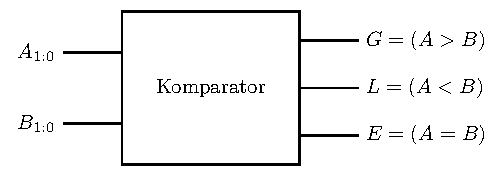
\includegraphics[width=0.48\linewidth]{Zadatak_3/komparator2}
\caption{Dvobitni komparator.}\label{fig:comp2}
\end{figure}

% Izvor DOCX: blok 135
\begin{enumerate}[label=\alph*),start=2,leftmargin=*]
\item Projektovati kombinacionu mrežu koja na izlazu generiše petobitni binarni broj određen funkcijom

\end{enumerate}


% Izvor DOCX: blok 136
\begin{equation}\label{eq:3.3.1}
\mathrm{RES}=\max\bigl(A,2B,\lfloor C/2\rfloor\bigr)
\end{equation}


% Izvor DOCX: blok 137
gde su A, B i C neoznačeni četvorobitni brojevi. Na raspolaganju su četvorobitni komparatori i potrebna logička kola.



% Izvor DOCX: blok 138
\subsubsection*{Rešenje:}


% Izvor DOCX: blok 139
a) Višu polovinu brojeva poredimo komparatorom H, a nižu komparatorom L. Ako su njihove zastavice $G$, $L$ i $E$ redom „veće“, „manje“ i „jednako“, važi
\[G=G_H+E_HG_L,\qquad E=E_HE_L,\qquad L=\overline{G+E}.\]
Realizacija je prikazana na slici~\ref{fig:comp4}. Završni NILI može se realizovati ILI kolom i NI kolom sa spojenim ulazima, pa se poštuje zadati skup kola.

% Izvor DOCX: blok 140
\begin{figure}[!htbp]\centering
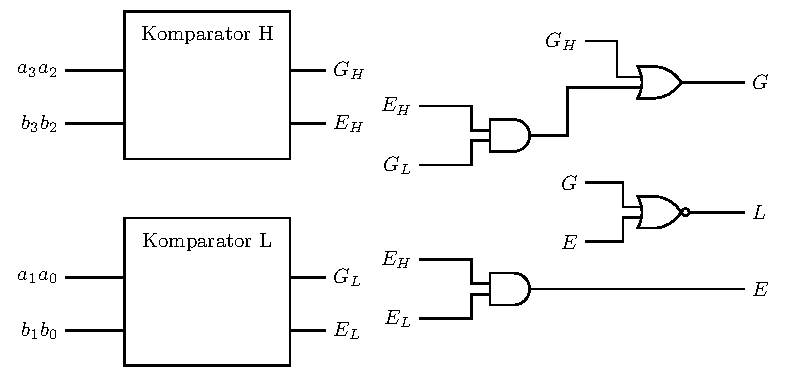
\includegraphics[width=0.9\linewidth]{Zadatak_3/komparator4}
\caption{Četvorobitni komparator od dva dvobitna komparatora.}\label{fig:comp4}
\end{figure}

% Izvor DOCX: blok 141
b) Neka je $X=A$, $Y=\lfloor C/2\rfloor$ i $Z=2B$. Prvi četvorobitni komparator i multiplekser određuju $M=\max(X,Y)$. Drugi poredi $M$ sa $Z_{3:0}$. Petobitni izlaz bira $Z$ kada je $Z_4=1$ ili $Z_{3:0}>M$, a inače bira $0M$. Tako visoki bit broja $2B$ ne može biti izgubljen.

% Izvor DOCX: blok 142
\begin{figure}[!htbp]\centering
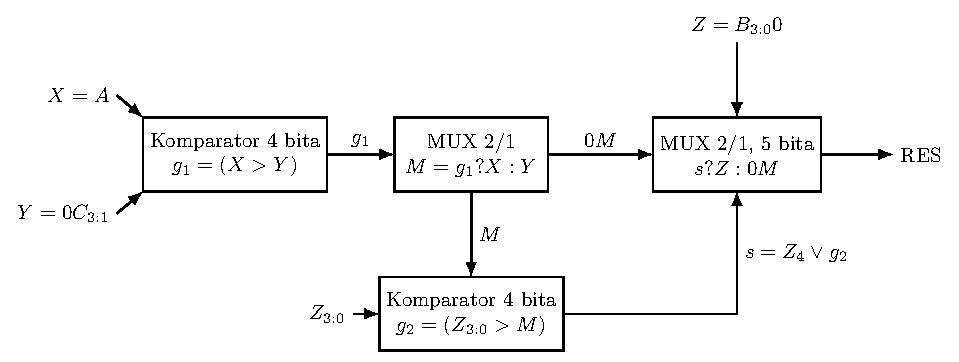
\includegraphics[width=0.9\linewidth]{Zadatak_3/maksimum}
\caption{Realizacija maksimuma tri neoznačene vrednosti.}\label{fig:max}
\end{figure}

% Izvor DOCX: blok 143
\FloatBarrier
\subsection{Zadatak 4}\label{sec:3.4}


% Izvor DOCX: blok 144
\begin{enumerate}[label=\alph*),leftmargin=*]
\item Realizovati sabirač dva neoznačena dvobitna broja $A=(a_1a_0)_2$ i $B=(b_1b_0)_2$, minimizovanjem izlaznih funkcija. Prikazati i realizaciju kada su dostupna XOR kola.
\item Korišćenjem sabirača iz tačke a realizovati funkciju:
\end{enumerate}

% Izvor DOCX: blok 145
\begin{equation}\label{eq:3.4.1}
Y = \ \left\{ \begin{array}{r}
(A + 1)(B + 1);A < B \\
2(A + 1)(B + 1);A > B \\
0;A = B
\end{array} \right.\
\end{equation}


% Izvor DOCX: blok 146
\subsubsection*{Rešenje:}


% Izvor DOCX: blok 147
a) Tabela~\ref{tab:adder} prikazuje sve ulazne kombinacije i zbir $S=A+B$.

% Izvor DOCX: blok 148
\begin{table}[!htbp]\centering\caption{Funkcionalna tabela dvobitnog sabirača.}\label{tab:adder}
\begin{tabular}{cccc|ccc}\toprule $a_1$&$a_0$&$b_1$&$b_0$&$s_2$&$s_1$&$s_0$\\\midrule
0&0&0&0&0&0&0\\
\redlinija
0&0&0&1&0&0&1\\
\redlinija
0&0&1&0&0&1&0\\
\redlinija
0&0&1&1&0&1&1\\
\redlinija
0&1&0&0&0&0&1\\
\redlinija
0&1&0&1&0&1&0\\
\redlinija
0&1&1&0&0&1&1\\
\redlinija
0&1&1&1&1&0&0\\
\redlinija
1&0&0&0&0&1&0\\
\redlinija
1&0&0&1&0&1&1\\
\redlinija
1&0&1&0&1&0&0\\
\redlinija
1&0&1&1&1&0&1\\
\redlinija
1&1&0&0&0&1&1\\
\redlinija
1&1&0&1&1&0&0\\
\redlinija
1&1&1&0&1&0&1\\
\redlinija
1&1&1&1&1&1&0\\
\bottomrule\end{tabular}\end{table}


% Izvor DOCX: blok 149
Iz tabele~\ref{tab:adder} popunjavamo Karnoove karte sa slike~\ref{fig:kmap}. Redovi su $a_1a_0$, a kolone $b_1b_0$, u Grejovom redosledu 00, 01, 11, 10.

% Izvor DOCX: blok 150
\begin{figure}[!htbp]\centering
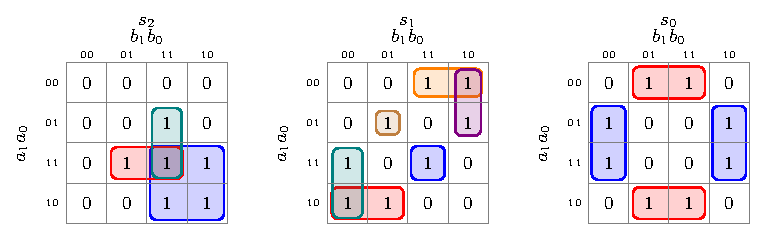
\includegraphics[width=\linewidth]{Zadatak_4/karno}
\caption{Karnoove karte za izlaze $s_2$, $s_1$ i $s_0$; obojene oblasti predstavljaju implicante.}\label{fig:kmap}
\end{figure}

% Izvor DOCX: blok 151
Grupisanjem jedinica dobijamo sledeće minimalne sume proizvoda:

% Izvor DOCX: blok 152
\begin{equation}\label{eq:3.4.2}
s_0=\bar a_0b_0+a_0\bar b_0
\end{equation}
\begin{equation}\label{eq:3.4.3}
\begin{aligned}s_1={}&a_1\bar a_0\bar b_1+a_1\bar b_1\bar b_0+\bar a_1\bar a_0b_1\\&+\bar a_1b_1\bar b_0+\bar a_1a_0\bar b_1b_0+a_1a_0b_1b_0.\end{aligned}
\end{equation}
\begin{equation}\label{eq:3.4.4}
s_{2} = \ b_{1}a_{1} + a_{1}a_{0}b_{0} + b_{1}b_{0}a_{0}
\end{equation}


% Izvor DOCX: blok 153
Kada su na raspolaganju XOR kola, dobijamo kompaktniju realizaciju. Zajednički signal $p_1=a_1\oplus b_1$ koristi se i za $s_1$ i za prenos:

% Izvor DOCX: blok 154
\begin{equation}\label{eq:3.4.5}
s_0=a_0\oplus b_0
\end{equation}
\begin{equation}\label{eq:3.4.6}
s_1=(a_1\oplus b_1)\oplus(a_0b_0)
\end{equation}
\begin{equation}\label{eq:3.4.7}
s_2=a_1b_1+(a_0b_0)(a_1+b_1)=a_1b_1+(a_0b_0)p_1
\end{equation}


% Izvor DOCX: blok 155
Na slici~\ref{fig:adder} prikazana je realizacija sa tri XOR, tri I i jednim ILI kolom. Ulazi su $A=(a_1a_0)_2$ i $B=(b_1b_0)_2$.

% Izvor DOCX: blok 156
\begin{figure}[!htbp]\centering
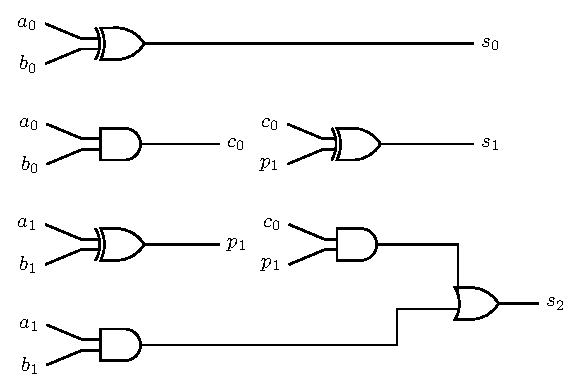
\includegraphics[width=0.9\linewidth]{Zadatak_4/sabirac}
\caption{Realizacija dvobitnog sabirača.}\label{fig:adder}
\end{figure}

% Izvor DOCX: blok 157
\begin{enumerate}[label=\alph*),start=2,leftmargin=*]
\item Funkciju \eqref{eq:3.4.1} možemo zapisati kao

\end{enumerate}


% Izvor DOCX: blok 158
\begin{equation}\label{eq:3.4.8}
Y=\begin{cases}X,&A<B,\\2X,&A>B,\\0,&A=B.\end{cases}
\end{equation}


% Izvor DOCX: blok 159
gde je X jednako:



% Izvor DOCX: blok 160
\begin{equation}\label{eq:3.4.9}
S=A+1,\qquad X=S(B+1)
\end{equation}


% Izvor DOCX: blok 161
Dakle, funkcija X se koristi i u slučaju $A > B$ i u slučaju $A < B$. U slučaju $A < B$ se koristi neizmenjena vrednost funkcije a u slučaju $A > B$ koristi se vrednost funkcije pomerena za 1 bit u levo dok se bit najmanje težine setuje na logičku nulu.



% Izvor DOCX: blok 162
Postoje mnogobrojni načini za realizaciju funkcije X, međutim, u ovom primeru će biti predstavljena realizacije funkcije X dobijena korišćenjem kola srednjeg stepena integracije.



% Izvor DOCX: blok 163
Funkciju X možemo posmatrati na sledeći način:



% Izvor DOCX: blok 164
\begin{equation}\label{eq:3.4.10}
B=0\quad\Longrightarrow\quad X=S
\end{equation}
\begin{equation}\label{eq:3.4.11}
B=1\quad\Longrightarrow\quad X=2S
\end{equation}
\begin{equation}\label{eq:3.4.12}
B=2\quad\Longrightarrow\quad X=3S
\end{equation}
\begin{equation}\label{eq:3.4.13}
B=3\quad\Longrightarrow\quad X=4S
\end{equation}


% Izvor DOCX: blok 165
Vrednost $B=(b_1b_0)_2$ bira jedan od ulaza $S,2S,3S,4S$ multipleksera 4/1. Pošto je $1\le S=A+1\le4$, maksimalne vrednosti ovih ulaza su 4, 8, 12 i 16. Zato svi podatkovni ulazi i izlaz multipleksera imaju pet bita; kraći zapisi dopunjavaju se vodećim nulama. Multiplekser je prikazan na slici~\ref{fig:mux4}.

% Izvor DOCX: blok 166
\begin{figure}[!htbp]\centering
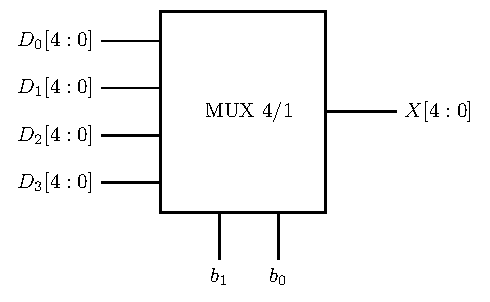
\includegraphics[width=0.5\linewidth]{Zadatak_4/mux4}
\caption{Multiplekser 4/1 sa petobitnim podatkovnim linijama.}\label{fig:mux4}
\end{figure}

% Izvor DOCX: blok 167
Ulazi $D_0=S$, $D_1=2S$ i $D_3=4S$ dobijaju se pomeranjem i dopunjavanjem nulama. Ulaz $D_2=3(A+1)$ može se dobiti i sabiranjem $S+2S$; ovde ga realizujemo direktno iz dvobitnog ulaza $A$, prema tabeli~\ref{tab:triS}.

% Izvor DOCX: blok 168
\begin{table}[!htbp]\centering\caption{Kodiranje $D_2=3(A+1)$.}\label{tab:triS}
\begin{center}\begin{adjustbox}{max width=\linewidth}
\begin{tabular}{ccccccc}\toprule
\emph{\textbf{a\textsubscript{1}}} & \emph{\textbf{a\textsubscript{0}}} & \emph{\textbf{D\textsubscript{2-4}}} & \emph{\textbf{D\textsubscript{2-3}}} & \emph{\textbf{D\textsubscript{2-2}}} & \emph{\textbf{D\textsubscript{2-1}}} & \emph{\textbf{D\textsubscript{2-0}}} \\
\midrule
0 & 0 & 0 & 0 & 0 & 1 & 1 \\
\redlinija
0 & 1 & 0 & 0 & 1 & 1 & 0 \\
\redlinija
1 & 0 & 0 & 1 & 0 & 0 & 1 \\
\redlinija
1 & 1 & 0 & 1 & 1 & 0 & 0 \\
\bottomrule\end{tabular}\end{adjustbox}\end{center}
\end{table}


% Izvor DOCX: blok 169
Iz tabele~\ref{tab:triS} dobijamo:

% Izvor DOCX: blok 170
\begin{equation}\label{eq:3.4.14}
D_{2,4}=0
\end{equation}
\begin{equation}\label{eq:3.4.15}
D_{2,3}=a_1
\end{equation}
\begin{equation}\label{eq:3.4.16}
D_{2,2}=a_0
\end{equation}
\begin{equation}\label{eq:3.4.17}
D_{2,1}=\bar a_1
\end{equation}
\begin{equation}\label{eq:3.4.18}
D_{2,0}=\bar a_0
\end{equation}


% Izvor DOCX: blok 171
Na slici~\ref{fig:x} prikazano je generisanje funkcije $X$.

% Izvor DOCX: blok 172
\begin{figure}[!htbp]\centering
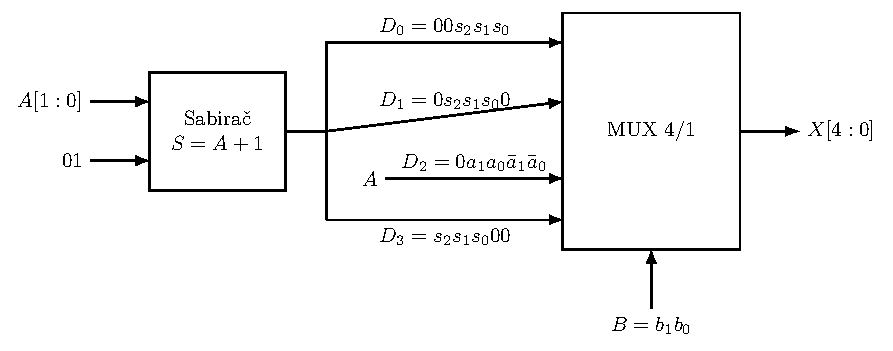
\includegraphics[width=0.9\linewidth]{Zadatak_4/proizvod}
\caption{Realizacija $X=(A+1)(B+1)$.}\label{fig:x}
\end{figure}

% Izvor DOCX: blok 173
Za konačan izlaz, šestobitni multiplekser bira $0X$ kada je $A\le B$, odnosno $X0=2X$ kada je $A>B$. Zatim se svih šest izlaznih bita maskira signalom $\overline{E}$, gde je $E=(A=B)$. Time je pri jednakosti izlaz nula, što je zasebna grana zadate funkcije. Šestobitna unutrašnja putanja omogućava neposredno pomeranje celog petobitnog $X$; za dozvoljene parove $A\ne B$ najveća izlazna vrednost je 24, pa je najviši izlazni bit uvek nula.

% Izvor DOCX: blok 174
Kompletna realizacija prikazana je na slici~\ref{fig:y}.

% Izvor DOCX: blok 175
\begin{figure}[!htbp]\centering
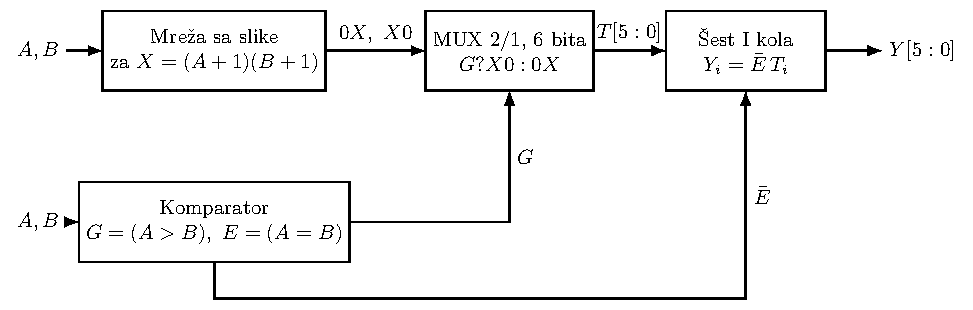
\includegraphics[width=0.9\linewidth]{Zadatak_4/kompletna}
\caption{Kompletna realizacija funkcije $Y$, uključujući granu $A=B$.}\label{fig:y}
\end{figure}

% Izvor DOCX: blok 176
\FloatBarrier
\subsection{Zadatak 5}\label{sec:3.5}


% Izvor DOCX: blok 177
\begin{enumerate}[label=\alph*),start=1,leftmargin=*]
\item Izvršiti sabiranje označenih brojeva datih u komplementu osnove ukoliko je na raspolaganju 5 cifara za predstavu rezultata. Operaciju sabiranja realizovati u brojnom sistemu u kome su brojevi i dati. Pored svakog rezultata naznačiti da li prilikom operacije sabiranja dolazi do prekoračenja

\end{enumerate}


% Izvor DOCX: blok 178
010\textsubscript{2} +0011\textsubscript{2}, 11\textsubscript{2} +110\textsubscript{2}, 0110\textsubscript{2} +1011\textsubscript{2}, 1100\textsubscript{2} +0101\textsubscript{2}, 0101\textsubscript{2} +0110\textsubscript{2}, 1101\textsubscript{2} +1011\textsubscript{2}, 1.0\textsubscript{2} +10.1\textsubscript{2}, 435\textsubscript{10} + 834\textsubscript{10}, A32F\textsubscript{16} + 476\textsubscript{16}, 324\textsubscript{7} + 365\textsubscript{7}



% Izvor DOCX: blok 179
\begin{enumerate}[label=\alph*),start=2,leftmargin=*]
\item Izvršiti oduzimanje označenih brojeva datih u komplementu osnove ukoliko je na raspolaganju 5 cifara za predstavu rezultata. Operaciju oduzimanja realizovati u brojnom sistemu u kome su brojevi i dati. Pored svakog rezultata naznačiti da li prilikom operacije oduzimanja dolazi do prekoračenja

\end{enumerate}


% Izvor DOCX: blok 180
010\textsubscript{2} -1101\textsubscript{2}, 11\textsubscript{2} -010\textsubscript{2}, 0110\textsubscript{2} -0101\textsubscript{2}, 1100\textsubscript{2} -1011\textsubscript{2}, 01.01\textsubscript{2} -10.10\textsubscript{2}, 1101\textsubscript{2} -0101\textsubscript{2}, 10\textsubscript{2} -011\textsubscript{2}, 435\textsubscript{10} - 166\textsubscript{10}, A32F\textsubscript{16} - 524\textsubscript{16}, 8135\textsubscript{16} - FA3B\textsubscript{16}, 364\textsubscript{7} - 302\textsubscript{7}



% Izvor DOCX: blok 181
\FloatBarrier
\subsection{Zadatak 6}\label{sec:3.6}


% Izvor DOCX: blok 182
\begin{enumerate}[label=\alph*),start=1,leftmargin=*]
\item Izvršiti sabiranje označenih brojeva datih u komplementu maksimalne vrednosti ukoliko je na raspolaganju 5 cifara za predstavu rezultata. Operaciju sabiranja realizovati u brojnom sistemu u kome su brojevi i dati. Pored svakog rezultata naznačiti da li prilikom operacije sabiranja dolazi do prekoračenja

\end{enumerate}


% Izvor DOCX: blok 183
010\textsubscript{2} +0011\textsubscript{2}, 11\textsubscript{2} +110\textsubscript{2}, 0110\textsubscript{2} +1011\textsubscript{2}, 1100\textsubscript{2} +0101\textsubscript{2}, 0101\textsubscript{2} +0110\textsubscript{2}, 1101\textsubscript{2} +1011\textsubscript{2}, 1.0\textsubscript{2} +10.1\textsubscript{2}, 435\textsubscript{10} + 834\textsubscript{10}, A32F\textsubscript{16} + 476\textsubscript{16}, 324\textsubscript{7} + 365\textsubscript{7}



% Izvor DOCX: blok 184
\begin{enumerate}[label=\alph*),start=2,leftmargin=*]
\item Izvršiti oduzimanje označenih brojeva datih u komplementu maksimalne vrednosti ukoliko je na raspolaganju 5 cifara za predstavu rezultata. Operaciju oduzimanja realizovati u brojnom sistemu u kome su brojevi i dati. Pored svakog rezultata naznačiti da li prilikom operacije oduzimanja dolazi do prekoračenja

\end{enumerate}


% Izvor DOCX: blok 185
010\textsubscript{2} -1101\textsubscript{2}, 11\textsubscript{2} -010\textsubscript{2}, 0110\textsubscript{2} -0101\textsubscript{2}, 1100\textsubscript{2} -1011\textsubscript{2}, 01.01\textsubscript{2} -10.10\textsubscript{2}, 1101\textsubscript{2} -0101\textsubscript{2}, 10\textsubscript{2} -011\textsubscript{2}, 435\textsubscript{10} - 166\textsubscript{10}, A32F\textsubscript{16} - 524\textsubscript{16}, 8135\textsubscript{16} - FA3B\textsubscript{16}, 364\textsubscript{7} - 302\textsubscript{7}



\end{document}
